
\gdef\commandfactory#1#2{%
   \global\expandafter\def\csname#1\endcsname{#1}
   \global\expandafter\def\csname#1caption\endcsname{#2}
}

\section{Four picture layouts}
\setlength{\columnsep}{0pt}

\begin{multicols}{2}
\normalsize
\textbf{Page layout.}\quad Four picture regular layouts, divide the page into a regular grid of four, as shown in Figure~\ref{fig:fourfigure}. They are the easiest to manipulate.
\smallskip
\fboxrule1pt
\par
\hspace{-20pt}\begin{minipage}{0.45\textwidth}\fbox{%
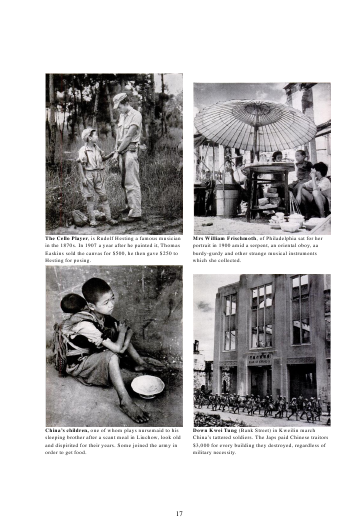
\includegraphics[width=\linewidth]{fourpicture}}\par
\captionof{figure}{Three figure layout, with a double column caption at the bottom figure.}
\label{fig:fourfigure}
\end{minipage}

\medskip

\lipsum
\fboxrule1pt
\medskip
\hskip-10pt\begin{minipage}{0.5\textwidth}\fbox{%
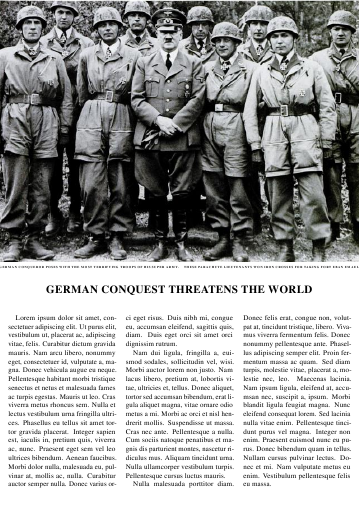
\includegraphics[width=\linewidth]{onepicture}}\par
\captionof{figure}{Three figure layout, with a double column caption at the bottom figure.}
\label{fig:fourfigure}
\end{minipage}
\smallskip
\end{multicols}
\clearpage







\vspace*{2cm}
\fbox{
\begin{minipage}[t]{\textwidth}
\begin{minipage}[t]{0.45\textwidth}
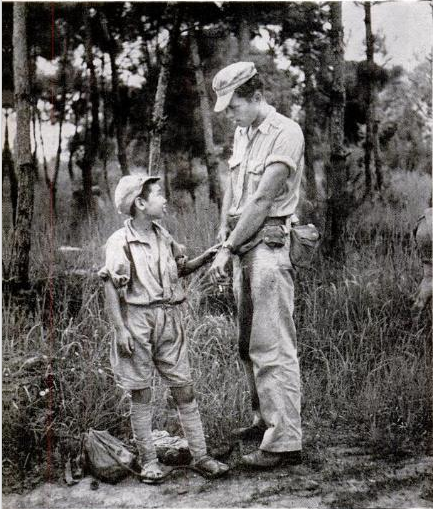
\includegraphics[width=1\textwidth]{china-01}\par\vspace*{-8pt}%
\captionof*{figure}{\noindent\footnotesize\textbf{The Cello Player}, is Rudolf Hesting a famous musician in the 1870s. In 1907 a year after
he painted it, Thomas Easkins sold the canvas for \$500, he then gave \$250 to Hesting for posing.}
\end{minipage}\hspace{0.5cm}
\begin{minipage}[t]{0.45\textwidth}
   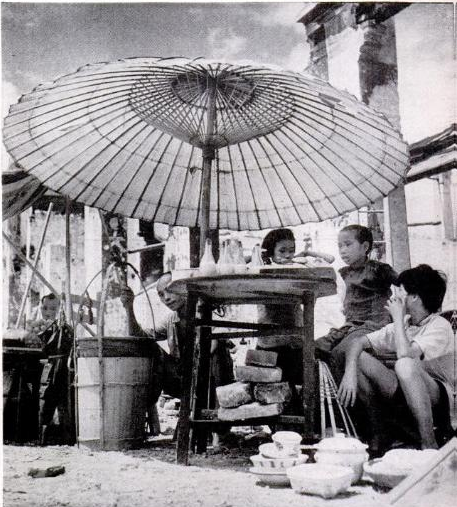
\includegraphics[width=1\textwidth]{china-02}\vspace*{-8pt}
    \captionof*{figure}{\noindent\footnotesize\textbf{Mrs William Frischmoth},
of Philadelphia sat for her portrait in 1900 amid a serpent, an oriental oboy, aa burdy-gurdy and other strange
musical instruments which she collected.}
\end{minipage}
\end{minipage}
}


\def\twoUp{%
\fbox{%
\begin{minipage}[t]{\textwidth}%
\begin{minipage}[t]{0.45\textwidth}%
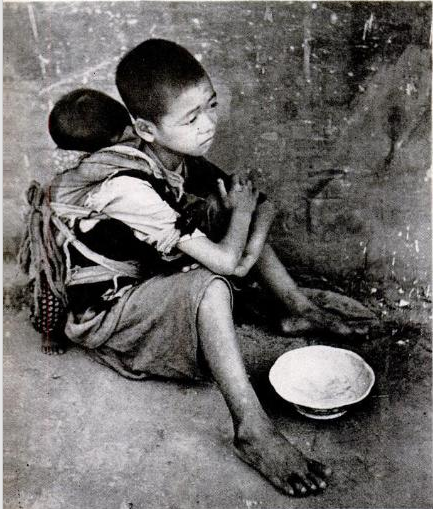
\includegraphics[width=1\textwidth]{china-03}\par\vspace*{-8pt}%
\captionof*{figure}{\footnotesize\textbf{China's children,} one of whom plays nursemaid to his sleeping
brother after a scant meal in Liuchow, look old and dispirited for their years. Some joined the army in order to get food.}%
\end{minipage}\hspace{0.5cm}
\begin{minipage}[t]{0.45\textwidth}
   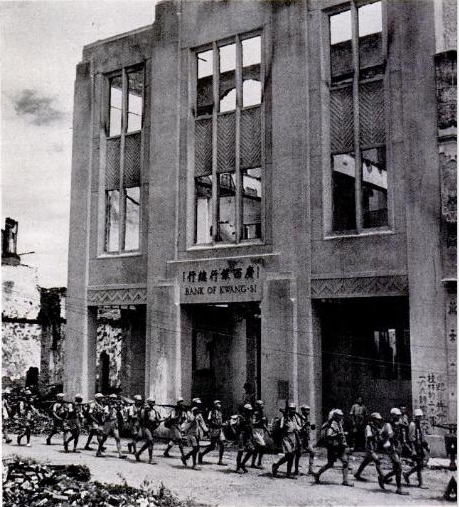
\includegraphics[width=1\textwidth]{china-04}\vspace*{-8pt}
   \captionof*{figure}{\noindent\footnotesize\textbf{Down Kwei Tung} (Bank Street) in Kweilin march China's tattered soldiers. The Japs paid Chinese traitors \$3,000 for every building they destroyed, regardless of military necessity. }
\end{minipage}
\end{minipage}
}
}

\twoUp

\vfill\vfill
\normalsize
\clearpage
.\par

\begin{minipage}[t]{0.22\textwidth}
   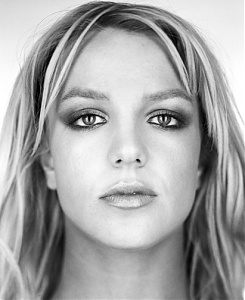
\includegraphics[width=1\textwidth]{britney_spears_2003}\vspace*{-8pt}
    \captionof*{figure}{\noindent\footnotesize\textbf{Down Kwei Tung} (Bank Street) in Kweilin march China's tattered soldiers. The Japs paid Chinese traitors \$3,000 for every building they destroyed, regardless of military necessity. }
\end{minipage}\hfill
\begin{minipage}[t]{0.22\textwidth}
   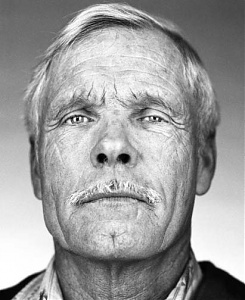
\includegraphics[width=1\textwidth]{ted_turner_2001}\vspace*{-8pt}
    \captionof*{figure}{\noindent\footnotesize\textbf{Down Kwei Tung} (Bank Street) in Kweilin march China's tattered soldiers. The Japs paid Chinese traitors \$3,000 for every building they destroyed, regardless of military necessity. }
\end{minipage}\hfill
\begin{minipage}[t]{0.22\textwidth}
   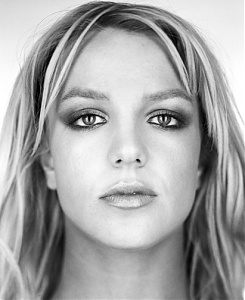
\includegraphics[width=1\textwidth]{britney_spears_2003}\vspace*{-8pt}
    \captionof*{figure}{\noindent\footnotesize\textbf{Down Kwei Tung} (Bank Street) in Kweilin march China's tattered soldiers. The Japs paid Chinese traitors \$3,000 for every building they destroyed, regardless of military necessity. }
\end{minipage}\hfill
\begin{minipage}[t]{0.22\textwidth}
   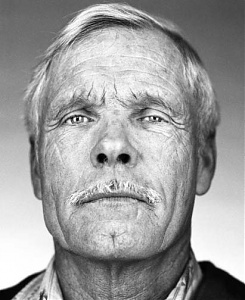
\includegraphics[width=1\textwidth]{ted_turner_2001}\vspace*{-8pt}
    \captionof*{figure}{\noindent\footnotesize\textbf{Down Kwei Tung} (Bank Street) in Kweilin march China's tattered soldiers. The Japs paid Chinese traitors \$3,000 for every building they destroyed, regardless of military necessity. }
\end{minipage}
\begin{minipage}[t]{0.22\textwidth}
   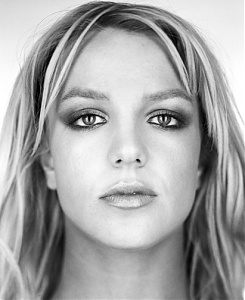
\includegraphics[width=1\textwidth]{britney_spears_2003}\vspace*{-8pt}
    \captionof*{figure}{\noindent\footnotesize\textbf{Down Kwei Tung} (Bank Street) in Kweilin march China's tattered soldiers. The Japs paid Chinese traitors \$3,000 for every building they destroyed, regardless of military necessity. }
\end{minipage}\hfill
\begin{minipage}[t]{0.22\textwidth}
   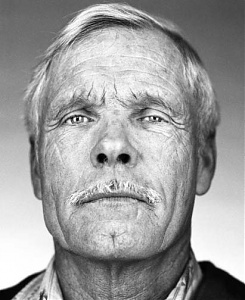
\includegraphics[width=1\textwidth]{ted_turner_2001}\vspace*{-8pt}
    \captionof*{figure}{\noindent\footnotesize\textbf{Down Kwei Tung} (Bank Street) in Kweilin march China's tattered soldiers. The Japs paid Chinese traitors \$3,000 for every building they destroyed, regardless of military necessity. }
\end{minipage}\hfill
\begin{minipage}[t]{0.22\textwidth}
   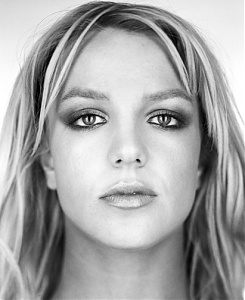
\includegraphics[width=1\textwidth]{britney_spears_2003}\vspace*{-8pt}
    \captionof*{figure}{\noindent\footnotesize\textbf{Down Kwei Tung} (Bank Street) in Kweilin march China's tattered soldiers. The Japs paid Chinese traitors \$3,000 for every building they destroyed, regardless of military necessity. }
\end{minipage}\hfill
\begin{minipage}[t]{0.22\textwidth}
   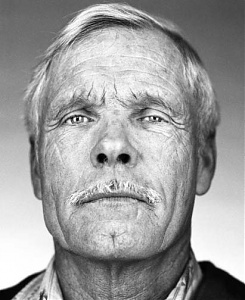
\includegraphics[width=1\textwidth]{ted_turner_2001}\vspace*{-8pt}
    \captionof*{figure}{\noindent\footnotesize\textbf{Down Kwei Tung} (Bank Street) in Kweilin march China's tattered soldiers. The Japs paid Chinese traitors \$3,000 for every building they destroyed, regardless of military necessity. }
\end{minipage}
\begin{minipage}[t]{0.22\textwidth}
   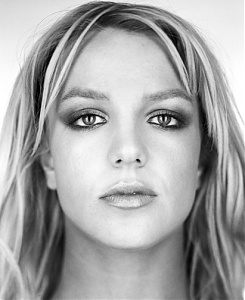
\includegraphics[width=1\textwidth]{britney_spears_2003}\vspace*{-8pt}
    \captionof*{figure}{\noindent\footnotesize\textbf{Down Kwei Tung} (Bank Street) in Kweilin march China's tattered soldiers. The Japs paid Chinese traitors \$3,000 for every building they destroyed, regardless of military necessity. }
\end{minipage}\hfill
\begin{minipage}[t]{0.22\textwidth}
   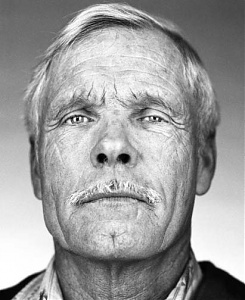
\includegraphics[width=1\textwidth]{ted_turner_2001}\vspace*{-8pt}
    \captionof*{figure}{\noindent\footnotesize\textbf{Down Kwei Tung} (Bank Street) in Kweilin march China's tattered soldiers. The Japs paid Chinese traitors \$3,000 for every building they destroyed, regardless of military necessity. }
\end{minipage}\hfill
\begin{minipage}[t]{0.22\textwidth}
   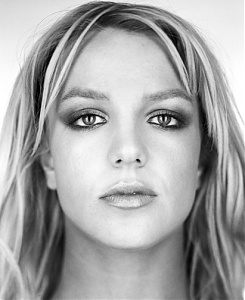
\includegraphics[width=1\textwidth]{britney_spears_2003}\vspace*{-8pt}
    \captionof*{figure}{\noindent\footnotesize\textbf{Down Kwei Tung} (Bank Street) in Kweilin march China's tattered soldiers. The Japs paid Chinese traitors \$3,000 for every building they destroyed, regardless of military necessity. }
\end{minipage}\hfill
\begin{minipage}[t]{0.22\textwidth}
   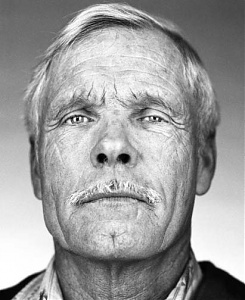
\includegraphics[width=1\textwidth]{ted_turner_2001}\vspace*{-8pt}
    \captionof*{figure}{\noindent\footnotesize\textbf{Down Kwei Tung} (Bank Street) in Kweilin march China's tattered soldiers. }
\end{minipage}

\bigskip

\hbox to \textwidth{\hfill\begin{minipage}{8.8cm}\captionof*{figure}{\noindent\footnotesize\textbf{Down Kwei Tung} (Bank Street) in Kweilin march China's tattered soldiers. The Japs paid Chinese traitors \$3,000 for every building they destroyed, regardless of military necessity. The Japs paid Chinese traitors \$3,000 for every building they destroyed, regardless of military necessity}\end{minipage}}

\clearpage
\newgeometry{top=1in,margin=1.8cm}
\lipsum
\clearpage
\pagebreak


\newgeometry{top=0cm,margin=1.5cm}
\def\heading{{\par \huge{\bf\centering \textsf{The \\Trouble With\\ Being Elfrida\\}}}}
\def\byline{{\par\bf \large{\textsf{Rich But Tense, Champion, can relax only if she loses.\\}}}}
\par
\fboxrule0pt
\fbox{%
\begin{minipage}[c][25cm][t]{0.3\textwidth}
\vspace*{2cm}
\underline{\textsf{PERSONALITY}}\par
\bigskip
\heading\par
\smallskip
\byline
\smallskip
\lorem\lorem\lorem\lorem
\medskip
\hfill\hfill\the\vsize
\end{minipage}}\hspace{25pt}%
\begin{minipage}[c][25cm][t]{0.70\textwidth}
\fbox{
 \centering
\hspace{0cm}\begin{minipage}[t]{0.70\textwidth}
  \centering
   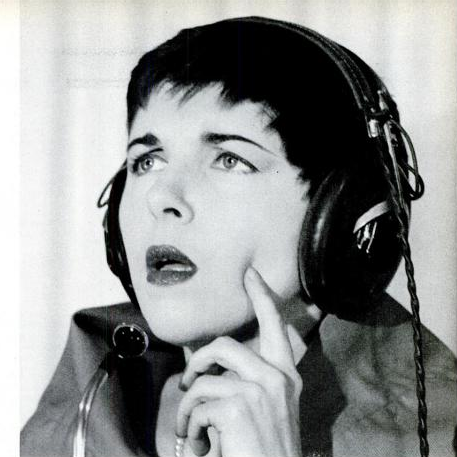
\includegraphics[width=0.5\textheight]{elfrida-top}
   \end{minipage}}\par
\smallskip\par
{\tiny \bf \RaggedRight\textsf{ ON TV ELFRIDA VON NARDROFF PONDERS MUSIC QUESTION (ABOVE). PREPARES (BELOW) TO ANSWER}}\par\smallskip
\fbox{%
\hspace{.8cm}\begin{minipage}[c]{0.7\textwidth}
   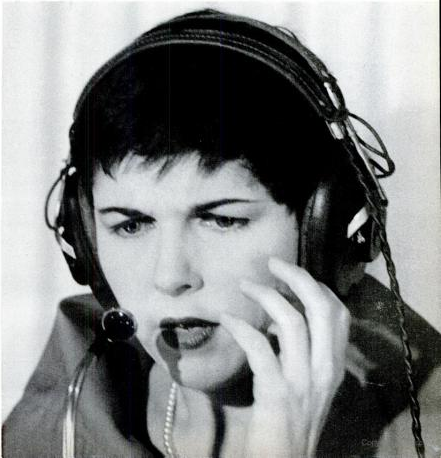
\includegraphics[height=.5\textheight]{elfrida-bottom}
\the\textheight June, 23, 1958
 \end{minipage}}
\end{minipage}

\clearpage
%% MEXICAN PAINTING
\newgeometry{top=0pt,left=0pt,bottom=0pt,margin=0pt}%
\fboxsep=0pt%
\fboxrule1pt%
\noindent\fbox{%
\begin{minipage}{\textwidth}%
\vspace*{0pt}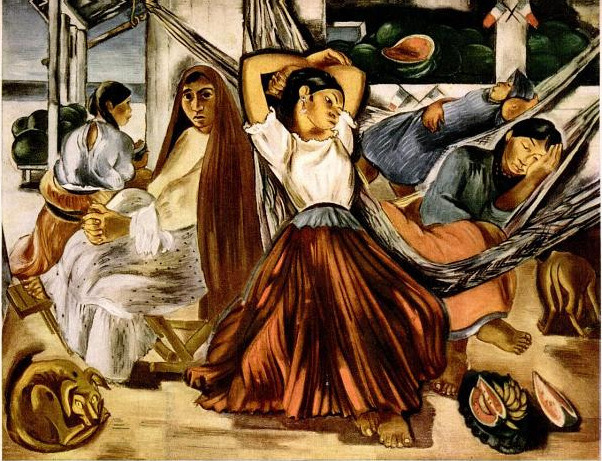
\includegraphics[width=\textwidth]{bythesea}\par
\vskip0pt\captionof{figure}{testing a bit more}\par
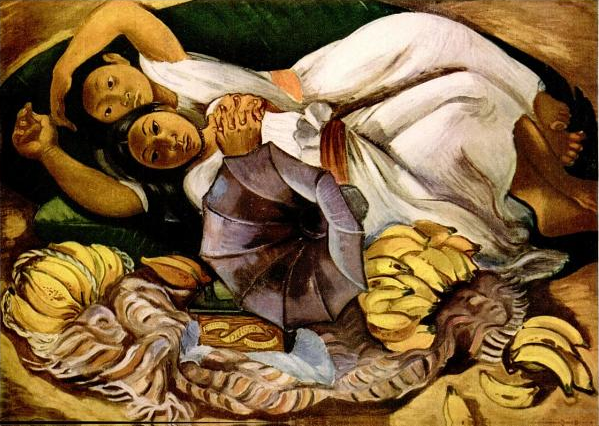
\includegraphics[width=\textwidth]{girlsandbananas}%
\end{minipage}}

\clearpage

\newcounter{noimages}
%% The environment image page, encloses its contents within a
%% minipage and acts as a real minipage, it scales everything based
%% on textwidth
%% 1  Scaling required
%%
\setcounter{noimages}{0}

%% We define the keys we are allowing in the environment
%% We define scale=0-1  a multiplier for linewidth
%%       pagestyle=string (one, two, three, four, five, six)
%%       align=center

\define@key{imgpg}{pagestyle}{\def\imgpg@pagestyle{#1}}
\define@key{imgpg}{scale}{\def\imgpg@scale{#1}}
\define@key{imgpg}{align}{\def\imgpg@align{#1}}
\define@key{imgpg}{top}{\def\imgpg@top{#1}}
\define@key{imgpg}{right}{\def\imgpg@right{#1}}
\define@key{imgpg}{bottom}{\def\imgpg@bottom{#1}}
\define@key{imgpg}{left}{\def\imgpg@left{#1}}
\define@key{imgpg}{geometry}{\def\imgpg@geometry{#1}}
%% We will probably need more keys but we will handle this later
%% Set defaults for all keys
\setkeys{imgpg}{pagestyle=one, scale=1, align=\centering, top=1in, right=1in, bottom=1in, left=1in}

%% We define the imagespage environment
%% Use as
%\begin{verbatim}
%% \begin{imagespage}[scale = 0.9, pagestyle = 2pic1]
%%     \addimagefromDB{}
%%     \addimagesfromDB{}
%%     \addcaptionfromDB{}
%% \end{imagespage}
%\end{verbatim}
\newenvironment{imagespage}[1][scale=1,pagestyle=one]{%
%%     we set the keys to their value
    \setkeys{imgpg}{#1}%
%%  adjust geometry
    \newgeometry{top=\imgpg@top,
                          right=\imgpg@right,
                          left=\imgpg@left,
                          bottom=\imgpg@bottom}

    \minipage{\imgpg@scale\textwidth}

    \imgpg@align

    \newcommand{\addimage}[2][width=\textwidth]{%
        \stepcounter{noimages}%
        \ifnum\thenoimages=1
             \putimage[##1]{##2}\par%
        \else
             \putimage[##1]{##2}\par%
        \fi
       }%
    }
   {\endminipage%
    \newpage%
     Number of images printed so far \thenoimages
    \setcounter{noimages}{0}
    \restoregeometry}


\begin{imagespage}[scale=0.9]
   \addimage{nudeattable}
   \captionof{figure}{This is tested using an environment. }\par
   \addimage{thesource}
 \end{imagespage}

\begin{imagespage}[scale=0.9]
     \addimage{bythesea}
     \addimage{girlsandbananas}
     \captionof{figure}{This is tested using an environment. }\par
\end{imagespage}

\commandfactory{boys}{tops a favorite game of Mexican children, absorbs Ram\'on and Pablito sons of Don\b{a} Luisa Pineda de melissio Sanchez in whose adobe house Aerist Doris Rosenthal lived in the town of Cher\'an in southwestern Mexico. For posing\cite{knuth98}, Doris paid Ram\'on and Pablito in Chickle and, when not in school or learning their catechism in church, they carried her painting materials for her wherever she went sketching. This picture was bought by Museum of Modern Art in 1941.}

\commandfactory{boers}{Looking more like their ancestors than themselves, six old boers gather to comapre whiskers.}
\commandfactory{boersbeards}{Looking for something}

\commandfactory{africacorps}{medics in afric aworls}


\begin{imagespage}[pagestyle=one, top=3cm,left=100pt, right=1cm, scale=0.80]
    \addimage{\boers}
    \captionof{figure}{\boerscaption}
    \addimage[width=17.5cm]{\boersbeards}
    \captionof{figure}{\boerscaption}
\end{imagespage}
\ClearShipoutPictureBG
\begin{imagespage}[pagestyle=one, top=1cm, right=1cm, scale=1.3, align=\centering]
    \addimage{\boys}
    \captionof{figure}{\boyscaption}
\end{imagespage}





\newpage

 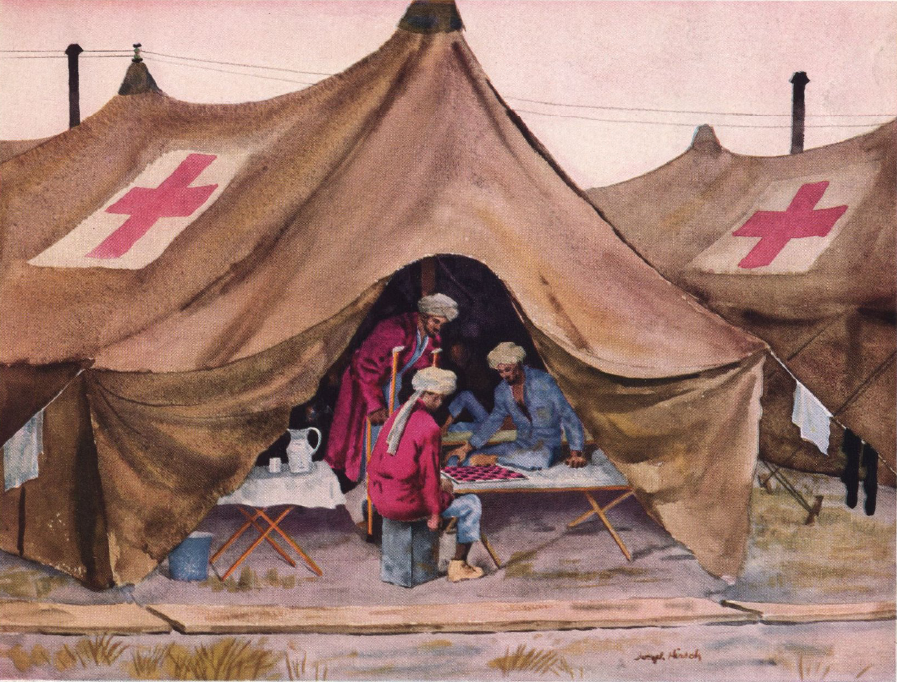
\includegraphics[height=0.95\textheight]{africamedics}

\hspace*{-\textwidth} 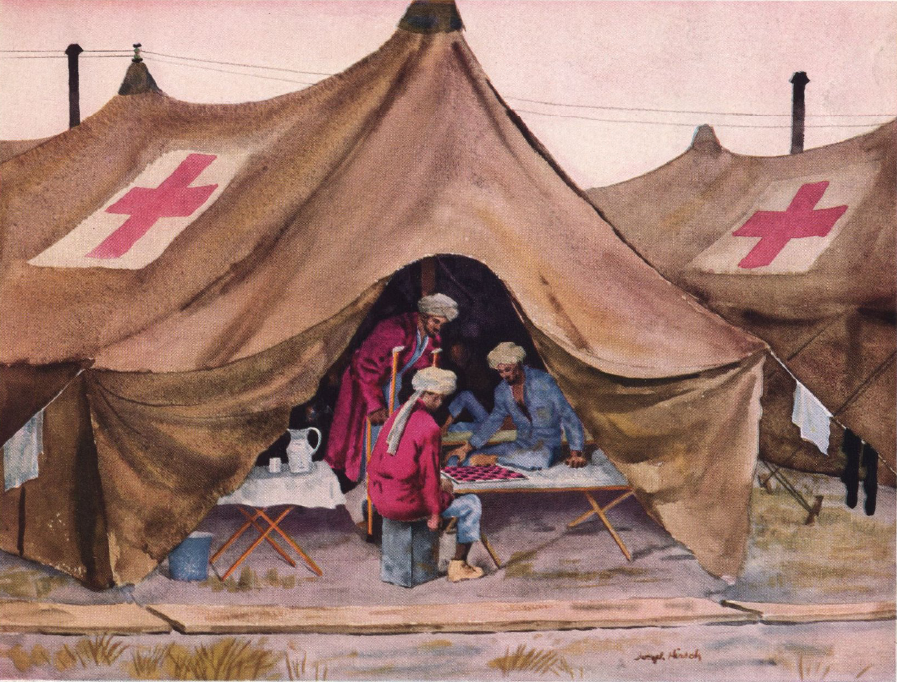
\includegraphics[height=0.95\textheight]{africamedics}

 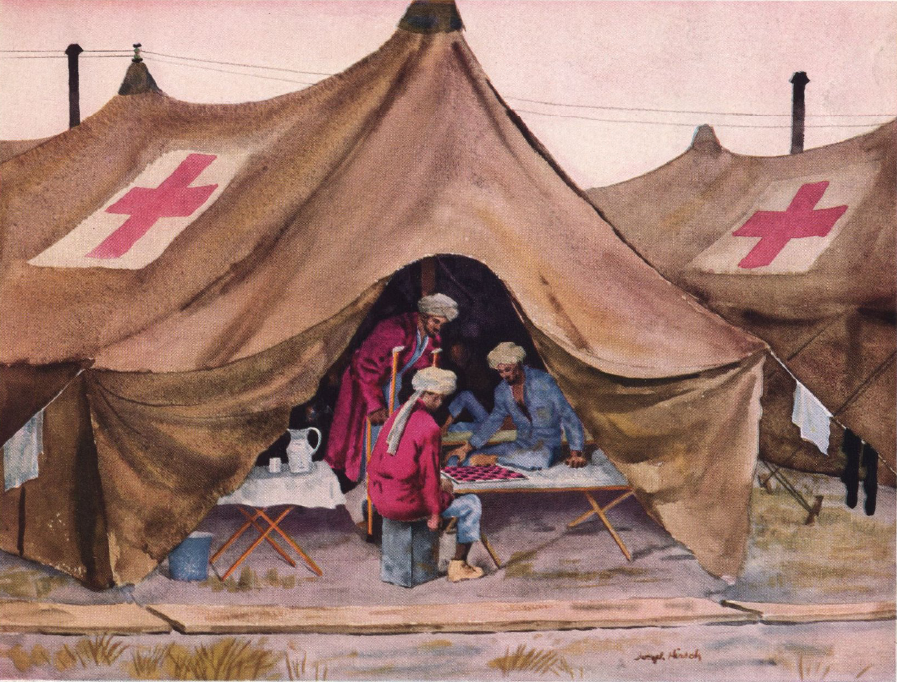
\includegraphics[height=0.95\textheight]{africamedics}

\hspace*{-\textwidth} 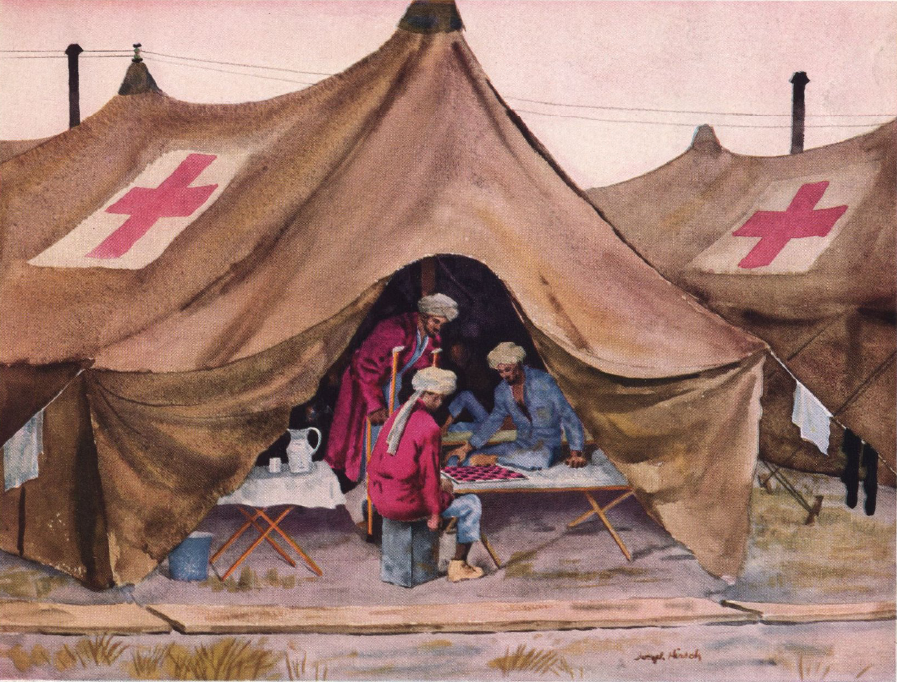
\includegraphics[height=0.95\textheight]{africamedics}

\restoregeometry

\cxset{toc image=\@empty}
\chapter{Centerfold}
Many photographs or pictures, might lose their appeal if printed at a small scale. many books spread these pictures over two pages, think of centerfolds.
\smallskip

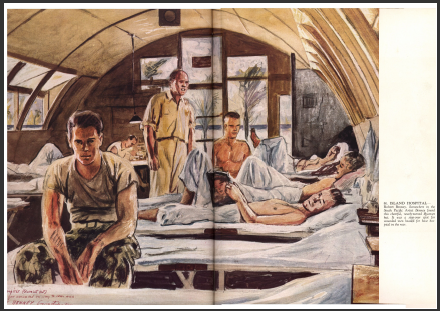
\includegraphics[width=0.9\linewidth]{spreadexample}

\smallskip

Although there is a package to do this, there is an easy way to achieve it and it needs two lines of code and perhaps a quad of calculation.


We include the same image on both pages and we set its height at the \verb!\textheight! or a slightly scaled dimension. We do the same for the second page except this time we shift it by textwidth. Assuming the picture is large enough placement can be achieved without any adjustments first time round..

{\footnotesize
\begin{verbatim}
\includegraphics[height=\textheight]{img}
\hspace*{\textwidth}
\includegraphics[height=\textheight]{img}
\end{verbatim}}

Minor scaling is inevitable to correct minor imperfections and this can be done on the second page.
Use the geometry package to adjust dimension.




We can include the images commands in minipages, if we need more control and easy scaling for both commands. We can also add a textblock to the second page. The textblock will need to be placed manually, but this is not difficult, if you use a minipage to enclose both the image as well as the textblock.
More involved macros can be obtained to automate the calculations, but to be honest it takes two or three runs to do this buy hand. If all the spreads are the same dimensions, you cann then have a reference to the x-shift, the y-shift might still need a bit of manipulation. For this we have provided an environment that automates the calculations.
\begin{verbatim}
\begin{twopagespread}[top=,left=,bottom=right=]
\putimage[keys]{img}
\puttextblock[keys]{text...}
\end{twopagespread}
\end{verbatim}





\newpage
\newgeometry{top=2cm,left=1cm,bottom=2cm}

\minipage{\textwidth}
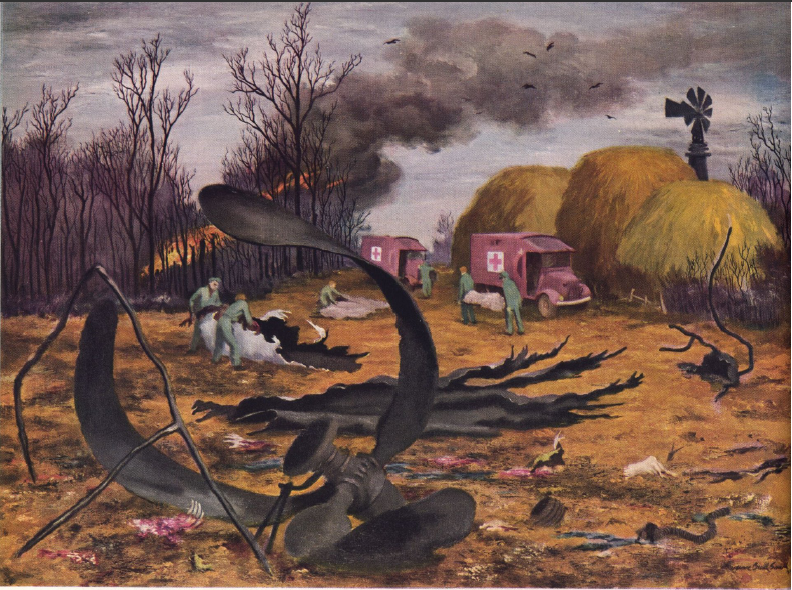
\includegraphics[height=\textheight]{deathofb2}
\endminipage

\hspace*{-1.07\textwidth}\minipage{\textwidth}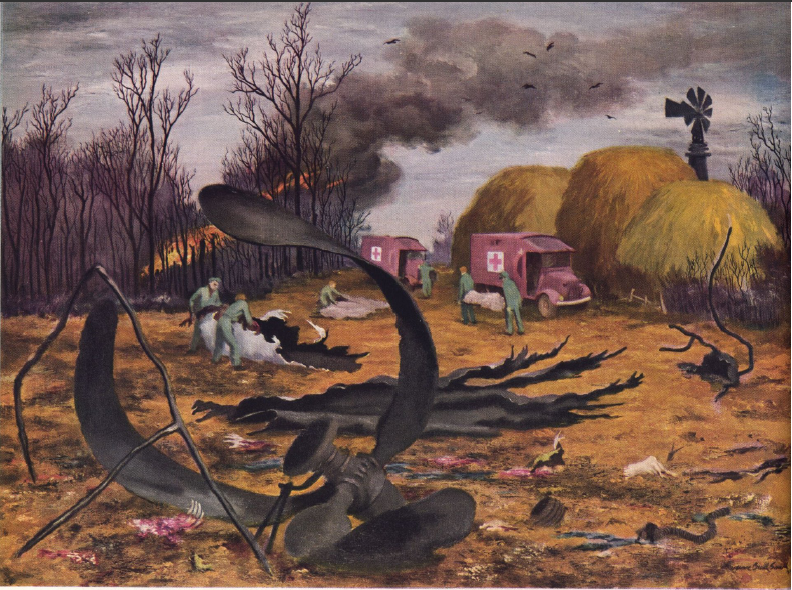
\includegraphics[height=\textheight]{deathofb2}
\endminipage

\minipage{\textwidth}
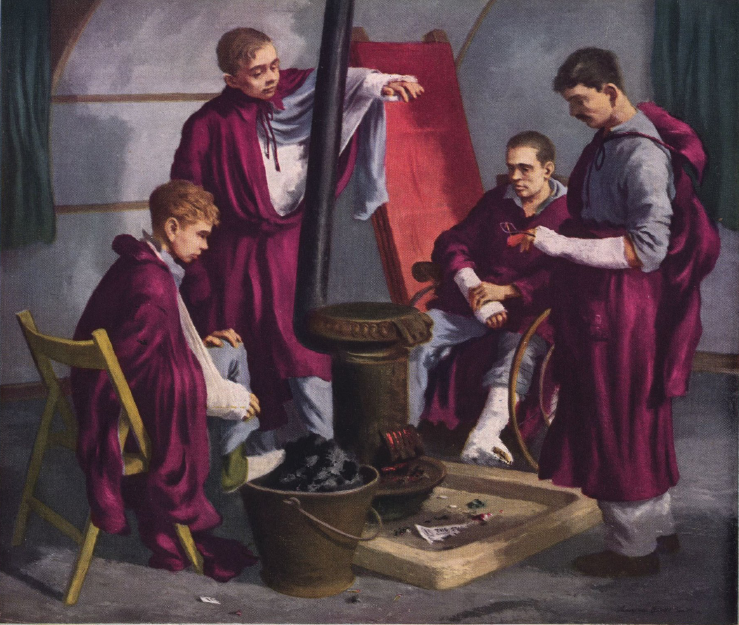
\includegraphics[height=\textheight]{firesidecomfort}
\endminipage

\hspace*{-1.12\textwidth}\minipage[t]{\textwidth}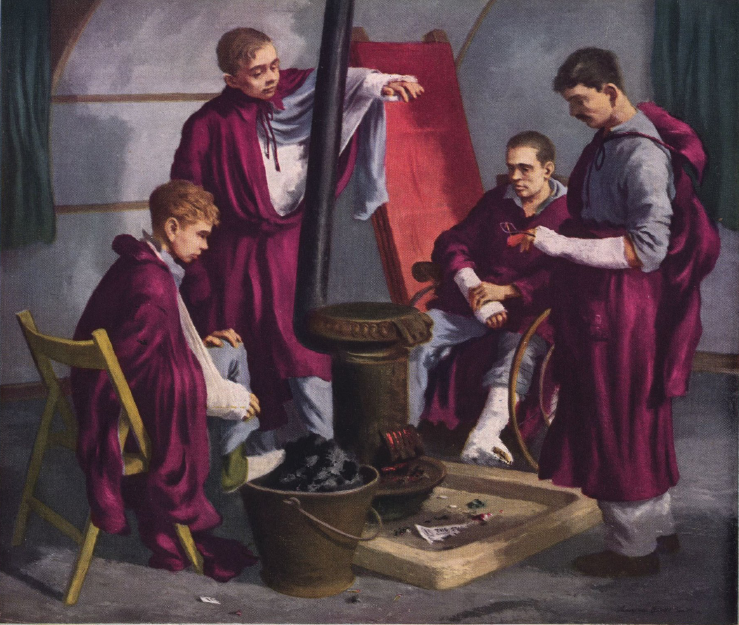
\includegraphics[height=\textheight]{firesidecomfort}
\endminipage

\vspace{-10cm}
\hspace*{11cm}\begin{minipage}[t]{4.5cm}
\lorem
\end{minipage}

\section{OVERFLOWING FIGURES INTO MARGINS}

Most users of \TeX\ are accustomed to let the system position images, either on top or bottom of the page and occasionally use the [h] positioning directive to place the image at the exact location it appears in the text. Traditional typography placed the image in many different positions. It also occasionally overflowed the image into the margins. The image below, copied from the \textit{American Antiquarian}, was placed in the original publication as such. Tufte advocates the use of such techniques in displaying not only information, but also other material such as tables. The Tufte class is discussed extensively in other sections. It has almost a religious following attached to it and I have personally used it for business reports.

\begin{figure}[htbp]
\leftskip-1.2cm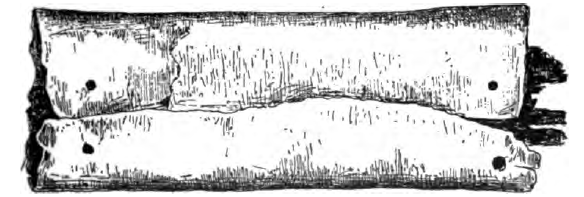
\includegraphics[scale=1.1]{copper-sheath}\par
\centerline{\textsc{Copper Sheath}}
\end{figure}

Almost as a matter of rule, the caption for these images was in small caps. Using small caps brought the caption into the easy attention of the reader, but it did not distract from the other elements of the page.
The image is not necessarily positioned symmetrically in the page, you can offset it to suit your taste, but in general, unless the image has any particular features that would make it look better offset rather than centered, is best positioned symmetrically. This can be automated, by writing a macro that measures the dimensions of the image and introduces a \verb+\leftskip+ so that the image can be shifted accordingly. A macro to achieve this is now described.


The image can be included by simply using a \verb+\skip-1.2cm+ or \verb+\leftskip-1.2cm+ :

\begin{verbatim}
\begin{figure}[htbp]
\leftskip-1.2cm\includegraphics{image}\par
\centerline{\textsc{Copper Sheath}}
\end{figure}
\end{verbatim}

